% Capitulo 2 - QEE e Disturbios elétromagneticos
\chapter{\capdois}\label{qeeDIS}

QEE é o principal tema motivador deste trabalho, no qual se aborda uma proposta de um sistema de tomada de decisões visando os parâmetros QEE em sistemas industriais. Precedendo maiores explanações sobre características de QEE e as perturbações elétricas, torna-se importante explicitar as definições literárias para esse conceito tão importante nos sistemas elétricos e neste trabalho.

\section{QEE e EE}\label{qeeEE}
\par 
A QEE é bem difundida e recebe diferentes definições que se justificam pelas diversificadas referências, pois concessionárias, consumidores e fabricantes de equipamentos têm diferentes pontos de vista em relação às definições deste termo \cite{FER99}.
\par 
Em \cite{DUG96} a qualidade da energia é definida como qualquer problema manifestado na tensão, corrente ou desvio de frequência, que resulte em falha ou má operação dos equipamentos dos consumidores. Segundo \cite{FER99}, QEE pode ser definida como a ausência relativa de variações de tensão provocadas pelo sistema da concessionária, particularmente a ausência de desligamentos, flutuações de tensão, transitórios e harmônicos medidos no ponto de entrega de energia. Esta é uma definição vista sob o enfoque da identificação de qual é o nível de qualidade da energia fornecida pela concessionária.
\par
Do ponto de vista do consumidor, a QEE pode ser definida como sendo a ausência de variações manifestadas na tensão, corrente ou frequência que resultem em falhas ou má operação de seus equipamentos \cite{DUG96}.
Segundo \cite{SBQEE}, citado por \cite{FER99}, uma abordagem acadêmica para QEE, sendo a disponibilidade da energia elétrica, com forma de onda senoidal e pura, sem alterações na amplitude, emanando de uma fonte de potência infinita. 
\par 
A Eficiência Energética está diretamente ligada a QEE, segundo \cite{INE12}, o Instituto Nacional de Eficiência Energética (INEE). Para se constatar se a eficiência energética é ou não obtida por uma ação, é preciso medir os resultados relacionados com a redução de consumo de energia e com os ganhos associados. Para se garantir que os resultados obtidos se mantenham ao longo do prazo contratual, é preciso verificar, por meio de monitoramento contínuo ou não, os seus valores.
\par
A Agência Nacional de Energia Elétrica (ANEEL) possui um plano de ação voltado a EE, nomeado de Programa de Eficiência Energética (PEE). Este plano é voltado para as empresas de distribuição de energia elétrica, mas também se aplicam neste trabalho no enfoque do melhoramento da eficiência energética ocasionada pelo emprego do sistema proposto. Para mais informações sobre o INEE e PEE podem ser consultadas as referências \cite{INE12} e \cite{ANEE3}.

\section{Normas Brasileiras}\label{qeenormas}
\par
No trabalho de \cite{JUN09}, é distinto que a padronização da QEE ainda se encontra em um estágio de desenvolvimento. A Europa é uma das regiões mais avançadas em relação à normalização da QEE, onde está vigente a EN50160. Já nos Estados Unidos, grande parte das concessionárias tem utilizado diversas normas como referência, como a IEEE 519. Entretanto, devido à desregulamentação existente, em contratos futuros à inclusão de cláusulas sobre a QEE devem se tornar padrões.
No cenário nacional, a QEE é monitorada pelas próprias concessionárias de energia elétrica, por meio de indicadores, que quantificam alguns distúrbios da QEE fornecida. Tais indicadores são definidos através das portarias e resoluções publicadas por órgãos reguladores, estabelecendo metas, ações e prazos a serem cumpridos pelas concessionárias a cada ano.
\par
A ANEEL, autarquia em regime especial vinculada ao Ministério de Minas e Energia, foi criada para regular o setor elétrico brasileiro, por meio da Lei nº 9.427/1996 e do Decreto nº 2.335/1997. A ANEEL iniciou suas atividades em dezembro de 1997, tendo como principais atribuições \cite{ANEEL}:
%% Itens em topicos
\begin{itemize}
\item Regular a produção, transmissão, distribuição e comercialização de energia elétrica;
\item Fiscalizar, diretamente ou mediante convênios com órgãos estaduais, as concessões, as permissões e os serviços de energia elétrica;
\item Implementar as políticas e diretrizes do governo federal relativas à exploração da energia elétrica e ao aproveitamento dos potenciais hidráulicos;
\item Estabelecer tarifas;
item Mediar, na esfera administrativa, os conflitos entre os agentes e entre esses agentes e os consumidores.
\end{itemize}
\par
Porem é delegação do governo federal, promover as atividades relativas às outorgas de concessão, permissão e autorização de empreendimentos e serviços de energia elétrica.

\par 
O documento \cite{MOD08} integra os Procedimentos de Distribuição de Energia Elétrica no Sistema Elétrico Nacional (PRODIST), juntamente com outros oito módulos. Esses documentos foram criados e são mantidos pela ANEEL, objetivando a normalização e padronização das atividades técnicas relacionadas ao funcionamento e desempenho dos sistemas de distribuição de energia elétrica, relacionados às distribuidoras, demais integrantes do sistema elétrico e alguns tópicos relevantes aos consumidores.
\par
As distribuidoras de energia são avaliadas em diversos aspectos no fornecimento de energia elétrica pela ANEEL, entre eles, está à qualidade do serviço e do produto oferecidos aos consumidores e fiscalização de concessionárias, permissionárias e autorizadas dos serviços de geração distribuída e de distribuição de energia elétrica. A qualidade dos serviços prestados compreende a avaliação das interrupções no fornecimento de energia elétrica. Destacam-se no aspecto da qualidade do serviço os indicadores de continuidade coletivos e os indicadores de continuidade individuais, são eles:
\begin{itemize}
\item Indicadores de continuidade coletivos:
	\begin{itemize}
		\item Duração equivalente de interrupção por unidade consumidora (DEC); 
		\item Frequência equivalente de interrupção por unidade consumidora (FEC).	
	\end{itemize}
\item Indicadores de continuidade individual:
	\begin{itemize}
		\item Duração de interrupção individual por unidade consumidora (DIC);
		\item Frequência de interrupção individual por unidade consumidora (FIC);
		\item Duração máxima de interrupção contínua por unidade consumidora ou ponto de conexão (DMIC).
	\end{itemize}
\end{itemize}
\par
O DEC exprime o espaço de tempo em que, em média, cada consumidor do conjunto considerado ficou privado do fornecimento de energia elétrica, o FEC representa o número de interrupções que, em média, cada consumidor do conjunto considerado foi atingido durante um determinado intervalo de tempo. DIC expressa o intervalo de tempo que, no período de apuração, em cada unidade consumidora ou ponto de conexão ocorreu descontinuidade da distribuição de energia elétrica, o FIC representa número de interrupções ocorridas, no período de apuração, em cada unidade consumidora ou ponto de conexão e o DMIC é o tempo máximo de interrupção contínua de energia elétrica, em uma unidade consumidora ou ponto de conexão.
\par 
A qualidade do produto avalia a conformidade de tensão em regime permanente e as perturbações na forma de onda de tensão. Destacam-se, neste quesito, os indicadores coletivos DRP e DRC, obtidos a partir da campanha de medição amostral instituída pela ANEEL dentro da respectiva área de concessão \cite{ANEE2}.

\section{Distúrbios Elétromagneticos}\label{dis}
\par 
Na literatura encontram-se diversificadas nomenclaturas objetivando a conceituação dos fenômenos descritos nos próximas capítulos, os termos distúrbios e perturbações são os mais difundidos nesses casos. 
\par 
Conforme explicado por \cite{FER99}, a ocorrência de distúrbios eletromagnéticos está relacionada a uma série de fatores identificados da operação normal de determinadas cargas ou dispositivos em um sistema elétrico, ou da ocorrência de fenômenos naturais que afetam o sistema elétrico.
\par 
Segundo \cite{JUN09}, os distúrbios que afetam a QEE podem ser originados tanto nos sistemas quanto nos equipamentos das concessionárias, ou ainda em última milha nos equipamentos dos consumidores. No entanto, as causas destes distúrbios em grande parte não estão no controle das concessionárias, pelo fato que se tratam de fenômenos gerados por causas aleatórias  (atividades de construção, acidentes e falhas no sistema elétrico), fenômenos naturais (relâmpagos, ventos, gelo, etc.) e as operações cotidianas da concessionária (chaveamentos, operações com banco de capacitores e manutenção) que pode gerar distúrbios para o sistema.
\par 
A Figura \ref{fig:tiposperturbações}, demonstra uma onda inicialmente sem perturbações, e a mesma com a aplicação de alguns dos mais ocorrentes distúrbios elétricos de tensão, tais distúrbios são explanados brevemente nesta seção \ref{qeeDIS}, onde destaca-se principalmente os Transitórios oscilatórios de baixa frequência, as variações de tensão de curta duração (VTCDs)e as distorções na forma de onda.
% Figura tipos de perturbações
\begin{figure}[hbt]
\begin{center}
% Nome da figura em cima, fonte abaixo
\caption{Distúrbios Elétricos}
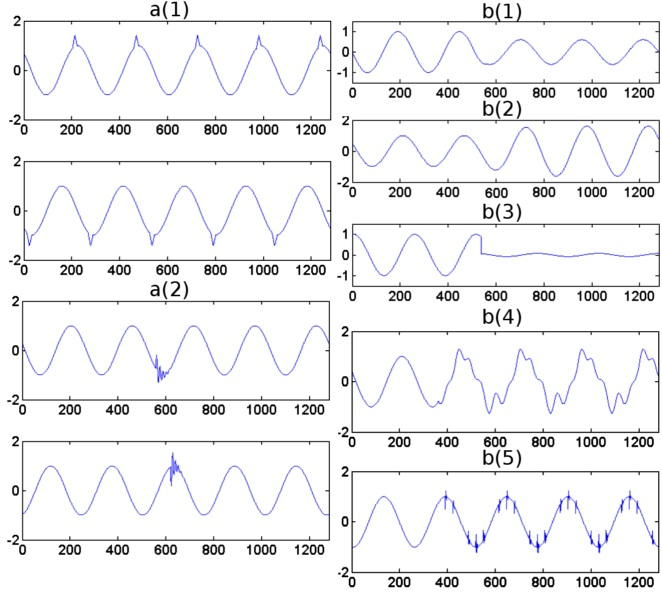
\includegraphics[width=12cm]{imagens/Imagema-final-AB2.jpg}
% Para que a fonte fique em tamanho 10
\par{\small Fonte: Ambas as imagens foram adaptadas pelo autor de \cite{FER10}.}
\label{fig:tiposperturbações}
\end{center}
\end{figure}
\par Distúrbios a e b
\begin{itemize}
\item a(1) Transitórios impulsivos
\item a(2) Transitórios oscilatórios
\item b(1) Afundamento de tensão
\item b(2) Elevação de tensão
\item b(3) Interrupção
\item b(4) Harmônicos 
\item b(5) Cortes
\end{itemize}
\subsection{Transitórios}
\par 
Fenômenos transitórios ocorrem no sistema elétrico em função de diversas condições. Muitos transitórios são decorrentes de variações instantâneas na corrente, as quais interagem com a impedância do sistema, resultando em elevadas tensões instantâneas.
\par 
Em \cite{IEE95}, citado por \cite{DEL03}, transitórios podem ser consequência de cargas com operação intermitente, chaveamento de bancos de capacitores, faltas a terra, operação de dispositivos de semicondutores e falhas em condutores. Descargas atmosféricas são um caso especial de transitórios, devido aos níveis extremamente altos de energia e rápido tempo envolvido.
\par 
A duração de um transitório é pequena, porém de grande importância, uma vez que os equipamentos presentes nos sistemas elétricos estarão submetidos a grandes solicitações de tensão e/ou corrente. Fenômenos transitórios podem ser classificados em dois grupos: os chamados transitórios impulsivos e os oscilatórios, causados por descargas atmosféricas e por chaveamentos respectivamente \cite{DEL03}

%Transitórios oscilatórios de baixa frequência
\par
Segundo \cite{BAC11}, os transitórios oscilatórios de baixa frequência (até 5 kHz), são bastante comuns na rede de distribuição. Na maioria das vezes são produzidos por chaveamento de bancos de capacitores ou energização de transformadores.
De acordo com \cite{JUN09}, citado por \cite{BAC11}, os transitórios são fenômenos eletromagnéticos oriundos de variações súbitas do valor instantâneo da tensão do sistema de energia elétrica. Em \cite{DEL03}, citado por \cite{BAC11}, é caracterizado por ser um evento indesejável com altas frequências em seu espectro e de curta duração, mas de vital relevância, já que submete os equipamentos a grandes solicitações tanto de tensão quanto de corrente. A intensidade do transitório depende da quantidade de energia armazenada no instante inicial do fenômeno e do comportamento transitório até o restabelecimento do novo ponto de operação do sistema.

\subsection{Variações de tensão de longa duração}
\par
As variações de tensão de longa duração podem ser caracterizadas como desvios que ocorrem no valor eficaz da tensão, na frequência do sistema, com duração maior que 1 minuto \cite{DUG96}.
\par 
Em \cite{DEL03}, estas variações acontecem como subtensões, sobretensões ou interrupções sustentadas, ambas são geralmente causadas por variações de carga e operações de chaveamento no sistema.
\par 
Já \cite{FER99} define as variações de longa duração englobando os desvios de valor eficaz de tensão, à frequência industrial, maiores que 1 minuto. Sobretensões e subtensões não são, geralmente, causadas por faltas no sistema, mas por variações de carga e operações de chaveamentos no sistema elétrico.

\subsection{Variações de tensão de curta duração}
\par 
Em \cite{DUG96}, conceitua-se as variações de tensão de curta duração apresentado duração típica entre 0,5 ciclo a 1 minuto, podendo ser subdivididas em alterações instantâneas, momentâneas ou temporárias, dependendo da duração do fenômeno. Tais variações de tensão são, geralmente, causadas por condições de falta, energização de grandes cargas, as quais requerem altas correntes de partida, ou por intermitentes falhas nas conexões dos cabos do sistema. 
\par 
Dependendo do local da falta e das condições do sistema, a falta pode causar tanto um afundamento de tensão, como uma elevação de tensão, ou mesmo uma interrupção completa do sistema elétrico.
\par 
As variações de tensão de curta duração são fenômenos que apresentam duração entre 0,5 ciclo até 1 minuto e podem ser caracterizadas por alterações instantâneas, momentâneas ou temporárias \cite{JUN09}. Tais alterações geralmente são ocasionadas por curtos circuitos no sistema elétrico e chaveamento de grandes cargas, demandam altas correntes ou perdas intermitentes da conexão com a rede. 
\par 
Tais eventos descritos, geram instabilidade ao sistema causando transtornos ao processo de produção por distorcer a forma de onda da tensão, podendo até interromper o abastecimento de energia elétrica caso não sejam tomadas as medidas preventivas. Dependendo do local da falha e das condições do sistema, o distúrbio resultante pode ser um afundamento de tensão, uma elevação de tensão ou uma interrupção do fornecimento de energia \cite{IEE95}. A seguir apresenta-se a descrição de cada um destes fenômenos.

\subsubsection{Afundamento de Tensão}
\par 
Afundamento de tensão é a terminologia mais utilizada no Brasil, na literatura internacional os termos correspondentes mais utilizados são voltage sage e voltage dip. Segundo \cite{FER99}, afundamentos de tensão consistem do decaimento de tensão ou corrente eficaz, à frequência industrial, para uma faixa entre 0,1 a 0,9 pu \footnote{Sistema por unidade.}, ocorrendo em um intervalo de 0,5 ciclo a 1 minuto, a duração dos afundamentos de tensão classifica-os entre três categorias: instantâneos, momentâneos e temporários.
\par 
As causas típicas para os afundamentos de tensão estão associadas à faltas no sistema em geral, grandes variações de carga e partidas de grandes motores. Quando há ocorrência de faltas no sistema, os afundamentos de tensão ocorrem devido à circulação de corrente de falta pela impedância do sistema, ocasionando uma queda de tensão no ponto de interesse, nestes casos os afundamentos têm seu tempo determinado por dispositivos de eliminação de faltas.
\par
Em \cite{OLIVE} e \cite{SIL01}, citados por \cite{DEL03}, o fenômeno de afundamento de tensão é uma subtensão de curta duração caracterizada por uma redução no valor eficaz da tensão, entre 0,1 e 0,9 pu, na frequência fundamental, com duração entre 0,5 ciclo e 1 minuto. Este tipo de distúrbio está associado, principalmente, a faltas em sistemas de transmissão e de distribuição. Mas pode também ser causado pela energização de grandes cargas, partida de grandes motores e pela corrente de energização de um transformador.
\par
O principal efeito destes distúrbios é o mau funcionamento dos equipamentos eletrônicos, em especial os computadores, que são alvo das preocupações de órgãos de pesquisa em QEE. Entretanto, determinar os níveis de sensibilidade de tais equipamentos torna-se uma tarefa difícil, devido ao grande número de medições necessárias para a coleta de dados, e ainda, as dificuldades de se ter equipamentos de medição em condições reais de campo \cite{OLIVE}, citado por \cite{DEL03}.

\subsubsection{Elevação de Tensão ou Salto de Tensão}
\par
Elevação de tensão ou Salto de tensão são as terminologias mais utilizadas no Brasil, na literatura internacional o termo correspondente mais utilizado é voltage swel. De acordo com \cite{FER99}, consiste no aumento da tensão ou corrente eficaz, à frequência industrial, para uma faixa entre 1,1 e 1,8 pu, ocorrendo em um intervalo de 0,5 ciclo a 1 min. A duração dos saltos de tensão classifica-os entre três categorias: instantâneos, momentâneos e temporários.
\par
Quando há ocorrência de faltas no sistema, os saltos de tensão ocorrem na fase não atingida pela falta. Nestes casos, a severidade do salto de tensão durante a condição de falta é determinada pela localização da falta, impedância do sistema e características de aterramento. Próximo à subestação haverá pouco ou nenhum salto de tensão pelo fato da usual conexão delta-estrela prover um caminho de baixa impedância de sequência zero para a corrente de falta. Segundo \cite{OLIVE}, citado por \cite{DEL03}, uma elevação de tensão é definida como um aumento entre 1,1 e 1,8 pu na tensão eficaz, para uma mesma frequência da rede, com duração entre 0,5 ciclo e 1 minuto.
\par
Assim como os afundamentos de tensão, as elevações de tensão estão geralmente associadas com as condições de falta no sistema, principalmente aos curtos circuitos fase-terra, visto que nestas condições as fases não defeituosas tendem a sofrer uma elevação de tensão.
\par
Este fenômeno pode também estar associado à saída de grandes blocos de cargas ou a energização de grandes bancos de capacitores, porém com uma incidência pequena se comparada com as sobretensões provenientes de faltas fase-terra nas redes de transmissão e distribuição \cite{DUG96}.
\par
No trabalho de \cite{DEL03} é relatado que as elevações de tensão são caracterizadas pelas suas magnitudes (valores eficazes) e suas durações. A severidade de uma elevação de tensão durante uma condição de falta é função do local da falta, da impedância do sistema e do aterramento do mesmo. A duração da elevação está intimamente ligada aos ajustes dos dispositivos de proteção, à natureza da falta (permanente ou temporária) e à sua localização na rede elétrica.
\par
Em situações de elevação de tensão oriundas de saídas de grandes cargas ou energização de grandes bancos de capacitores, o tempo de duração das elevações depende da resposta dos dispositivos reguladores de tensão das unidades geradoras, do tempo de resposta dos transformadores de tap variável e da atuação de compensadores síncronos que porventura existam no sistema. As consequências de elevações de tensão em aparelhos de iluminação, por exemplo, pode ser o aumento da luminosidade; já em um banco de capacitores pode, frequentemente, causar sérios danos ao equipamento.
\par
Dentro do exposto, a preocupação principal recai sobre os equipamentos eletrônicos, uma vez que estas elevações podem vir a danificar os componentes internos destes equipamentos, conduzindo-os à má operação, ou em casos extremos, à completa inutilização.

\subsubsection{Interrupção}
\par
Uma interrupção de curta duração ocorre quando a tensão de suprimento decresce para um valor menor que 0,1 pu por um período de tempo não superior a 1 minuto. Este tipo de interrupção pode ser causada por faltas no sistema de energia, falhas de equipamentos e mau funcionamento de sistemas de controle \cite{OLIVE}, citado por \cite{DEL03}.
\par
Algumas interrupções podem ser precedidas por um afundamento de tensão quando estas são devidas a faltas no sistema supridor. O afundamento de tensão ocorre no período de tempo entre o início de uma falta e a operação do dispositivo de proteção do sistema.
\par
Com o crescente emprego de cargas eletrônicas, como inversores e computadores, e com as faltas em redes aéreas sendo de natureza temporária, estas são responsáveis pela saída de operação de diversos equipamentos, interrompendo o processo produtivo e causando enormes prejuízos às indústrias \cite{DEL03}.
\par
Em \cite{FER99}, uma interrupção rápida é caracterizada quando a tensão eficaz da fonte ou a corrente de carga decresce a menos que 0.1 pu, por um período de tempo entre 0,5 ciclo e 1 minuto. As interrupções rápidas são resultado de faltas no sistema, falhas em equipamentos e mau funcionamento de dispositivos de controle.
\par
Tais interrupções quando causadas por faltas no sistema da concessionária, têm seu tempo determinado pelo tempo de operação de dispositivos de proteção do sistema elétrico (religadores). Quando causadas por mau funcionamento de equipamentos ou por falhas de conexões, têm um período de tempo irregular.

\subsection{Distorções da Forma de Onda}
\par 
A definição de \cite{OLIVE}, citado por \cite{DEL03} para uma distorção da forma de onda, é que a mesma pode ser um desvio, em regime permanente, da forma de onda puramente senoidal, na frequência fundamental, e é caracterizada principalmente pelo seu conteúdo espectral. Existem quatro principais tipos de distorções da forma de onda, descritos a seguir \cite{DUG96}.
\subsubsection{Harmônicos}
\par
Harmônicas são tensões ou correntes senoidais de frequências múltiplas inteiras da frequência fundamental na qual opera o sistema de energia elétrica. Estes harmônicos distorcem as formas de onda da tensão e corrente e são oriundos de equipamentos e cargas com características não lineares instalados no sistema de energia. 
\par
As distorções harmônicas estão em desacordo com os objetivos da qualidade de suprimento promovido por uma concessionária de energia elétrica, a qual deve fornecer aos seus consumidores uma tensão puramente senoidal, com amplitude e frequência constantes. \par
\par
Entretanto, o fornecimento de energia a determinados consumidores que causam deformações no sistema supridor prejudica não apenas o consumidor responsável pelo distúrbio, mas também outros conectados à mesma rede elétrica \cite{DEL03}.
\par
De acordo com \cite{FER99}, harmônicos são correntes ou tensões senoidais de frequências múltiplas (de inteiros) da frequência que o sistema é designado a operar. Sendo esses componentes harmônicos, combinados com a tensão ou corrente fundamentais, produzindo alterações na forma de onda. 
\par
A distorção harmônica existe devido a características não lineares de dispositivos e cargas do sistema elétrico. Já a distorção de tensão resulta da queda de tensão provocada pela passagem de corrente (injetada por uma carga não linear) pela impedância do sistema.
\par
Destacado por \cite{DUG96}, citado por \cite{FER99}, a importância da existência de uma distorção harmônica, sendo fenômeno que deve ser tratado como de regime permanente. A distorção de forma de onda, provocada pelos componentes harmônicos, deve estar presente, continuamente, por pelo menos alguns segundos.

\subsubsection{Interharmônicos, Ruídos e Nível Corrente Contínua (CC)}
\par
Interharmônicos são componentes de frequência, em tensão ou corrente, que não são múltiplos inteiros da frequência fundamental do sistema supridor (50 ou 60Hz\footnote{Hertz, unidade derivada do Sistema Internacional de Unidades (SI).}). Elas podem aparecer como frequências discretas ou como uma larga faixa espectral.
\par
Os interharmônicos podem ser encontrados em redes de diferentes classes de tensão. As suas principais fontes são conversores estáticos de potência, ciclo conversores, motores de indução e equipamentos a arco \cite{DEL03}.
\par
Ruído é definido por \cite{OLIVE}, citado por \cite{DEL03}, como um sinal elétrico indesejado, contendo uma larga faixa espectral com frequências menores que 200 kHz, as quais são superpostas às tensões ou correntes de fase, ou encontradas em condutores de neutro em linhas de transmissão.
\par
De acordo com \cite{DUG96}, os ruídos são basicamente uma distorção indesejada no sinal elétrico que não pode ser classificado como distorção harmônica ou transitório. A faixa de frequência e o nível da amplitude dependem da fonte que produz o ruído e das características do sistema. 
\par
A amplitude típica é menor que 1\% da tensão fundamental, e os mesmos podem causar distúrbios em equipamentos eletrônicos, tais como microcomputadores e controladores programáveis. O problema pode ser minimizado utilizando-se filtros, transformadores isoladores e alguns condicionadores de linha.
\par
A presença de tensão ou corrente CC em um sistema elétrico com corrente alternada (CA) é denominado \emph{DC offset}. Este fenômeno pode ocorrer como resultado da operação ideal de retificadores de meia-onda \cite{OLIVE}.
\par
O nível CC em redes de corrente alternada pode levar à saturação de transformadores, resultando em perdas adicionais e redução da vida útil. Pode também causar corrosão eletrolítica dos eletrodos de aterramento e de outros conectores \cite{DEL03}.
\subsubsection{Flutuações ou Oscilações de Tensão}
\par
No trabalho de \cite{DEL03} existe uma rápida explicação sobre as principais ocorrências sobre o assunto. As flutuações de tensão correspondem a variações sistemáticas dos valores eficazes da tensão de suprimento dentro da faixa compreendida entre 0,95 e 1,05 pu. Tais flutuações são geralmente causadas por cargas industriais e manifestam-se de diferentes formas.
\par
A principal fonte das Flutuações Aleatórias são os fornos a arco, onde as amplitudes das oscilações dependem do estado de fusão do material, bem como do nível de curto-circuito da instalação.
\par\textbf{Flutuações Repetitivas}
\par Dentre as principais fontes geradoras de flutuações desta natureza tem-se: Máquinas de solda, Elevadores de minas, Ferrovias.
\par\textbf{Flutuações Esporádicas}
\par A principal fonte causadora destas oscilações é a partida direta de grandes motores. Os principais efeitos nos sistemas elétricos, resultados das oscilações causadas pelos equipamentos mencionados anteriormente são:
\begin{itemize}
\item Oscilações de potência e torque das máquinas elétricas;
\item Queda de rendimento dos equipamentos elétricos;
\item Interferência nos sistemas de proteção;
\item Efeito Flicker ou cintilação luminosa.
\end{itemize}

\subsection{Desequilíbrios de Tensão}
\par
De acordo com \cite{DUG96}, os desequilíbrios de tensão podem ser caracterizados como a relação entre a componente de sequência negativa pela componente de sequência positiva dos sinais de correntes ou tensões trifásicas.
\par
As origens destes desequilíbrios estão geralmente nos sistemas de distribuição, os quais possuem cargas monofásicas distribuídas inadequadamente, fazendo surgir no circuito tensões de sequência negativa. Este problema se agrava quando consumidores alimentados de forma trifásica possuem uma má distribuição de carga em seus circuitos internos, impondo correntes desequilibradas no circuito da concessionária. Tensões desequilibradas pode ser também o resultado da queima de fusíveis em uma fase de um banco de capacitores trifásicos.
\par
Ambos os fatores interferem diretamente na QEE sobre o ponto de vista do fornecimento de energia idealizado inicialmente pela concessionária, mas esta qualidade é prejudicada por esses fatores e alguns consumidores têm em suas alimentações um desequilíbrio de tensão, o qual se manifesta sob três formas distintas: amplitudes diferentes, assimetria nas fases e assimetria conjunta de amplitudes e fases. Destas, apenas a primeira é frequentemente evidenciada no sistema elétrico.

\subsection{Variações na Frequência do Sistema Elétrico}
\par
Variações na frequência de um sistema elétrico são definidas como sendo desvios no valor da frequência fundamental deste sistema. No Brasil a frequência fundamental é de 60hz \cite{DUG96}. A frequência do sistema de potência está diretamente associada à velocidade de rotação dos geradores que suprem o sistema.
\par
Variações de frequência que ultrapassam os limites para operação normal em regime permanente podem ser causadas por faltas em sistemas de transmissão, saída de um grande bloco de carga ou pela saída de operação de uma grande fonte de geração.
\par
Em sistemas isolados, entretanto, como é o caso da geração própria nas indústrias, na eventualidade de um distúrbio, a magnitude e o tempo de permanência das máquinas operando fora da velocidade, resultam em desvios da frequência em proporções mais significativas.
\par
Na Tabela \ref{fig:tabpdistele} estão dispostos os tipos de distúrbios elétricos, classificados juntamente com suas principais causas de ocorrência e tempo de duração típica. Para o melhor entendimento das informações apresentadas na Tabela \ref{fig:tabpdistele}, consultar o Glossário.%\ref{gloss}. \cite{gloss} 
% tabela 1
% Obs o [!h] é para fixar a imagem exatamente neste ponto do texto
%Logo de seguida temos a possibilidade de introduzir um conjunto de opções entre []. São elas:
%h – Para que a imagem fique exactamente na parte do texto em que é introduzida (here);
%t – Para a imagem aparecer no topo da página (top);
%b – Para a imagem aparecer no fundo da página (bottom);
%p – Para a imagem aparecer numa página só com figuras ou tabelas.
\begin{table}[!h]
\begin{center}
\caption{Principais causas dos fenômenos eletromagnéticos conforme recomendação \cite{IEE95}.}
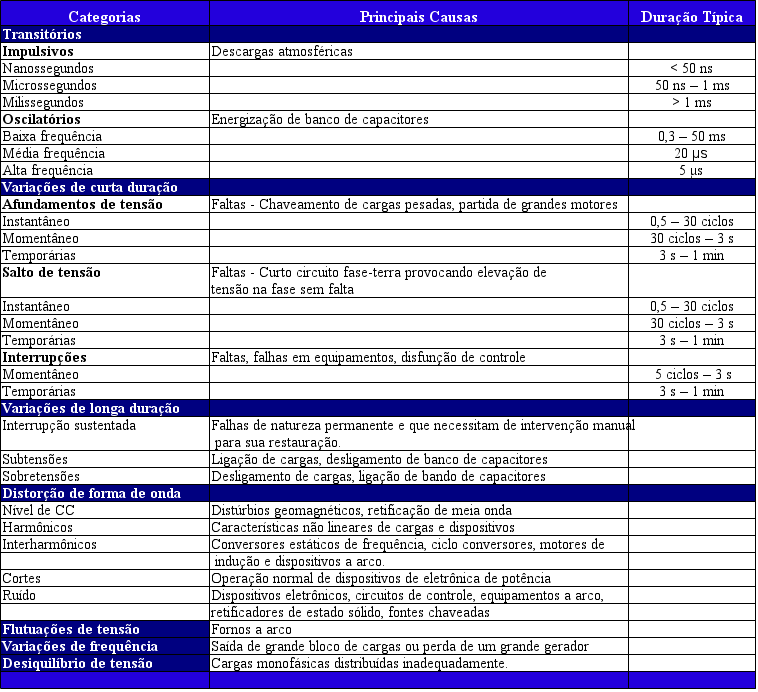
\includegraphics[height=15cm]{imagens/tab1_cap2.png}
\par{\small Fonte: Adaptada pelo autor de \cite{JUN09}.}
\label{fig:tabpdistele}
\end{center}
\end{table}
\section{Quantificação de QEE (Causas, Origens e Efeitos)}
\par
De acordo com \cite{ALV10}, distúrbios de energia elétrica ocorrem desde o inicio da concepção de sistemas elétricos de potência, e com o transcorrer dos anos desde o Séc. XIX, as cargas cada vez mais adquiriram sensibilidade a esses distúrbios e em consequentemente surgiu à necessidade de que a energia elétrica possuísse maior qualidade.
\par
As cargas sensíveis, como equipamentos eletrônicos, os microprocessados, Acionamentos a Velocidade Variável (AVVs), Controladores Lógicos Programáveis (CLPs), dentre outros são cada vez mais numerosas nos setores: industrial, comercial e residencial e, o nível de QEE requerido tem aumentado muito nos últimos anos. 
\par De forma que a energia passou a ser vista como um produto e não mais como um serviço, e como todo produto, passa a ser analisado pela sua qualidade e preço. Muitos consumidores não sabem a que tipo de distúrbios da QEE estão sendo expostos, basicamente por dois grandes motivos, pelo fato que os estudos e o trabalho de conscientização a população a respeito dos problemas de QEE são recentes. 
\par
De forma utópica o equilíbrio esperado entre as expectativas dos consumidores e as limitações das concessionárias, seria que estas poderiam informar sobre a QEE entregue, e conhecer as expectativas dos consumidores ligadas aos prejuízos causados pelos distúrbios da QEE.
\par
No entanto não é desta forma que a relação entre concessionárias e consumidores acontece, e os resultados ficam explícitos em prejuízos associados à QEE, dentre as diversas perturbações elétricas causadores de problemas de QEE, destacam-se os afundamentos de tensão e os harmônicos. As tabelas \ref{fig:tabpertcons} e \ref{fig:tabperdas} ilustram esta afirmação.
% tabela 2
\begin{table}[!h]
\begin{center}
\caption{Perturbações mais Comuns: Causas e Equipamentos Afetados}
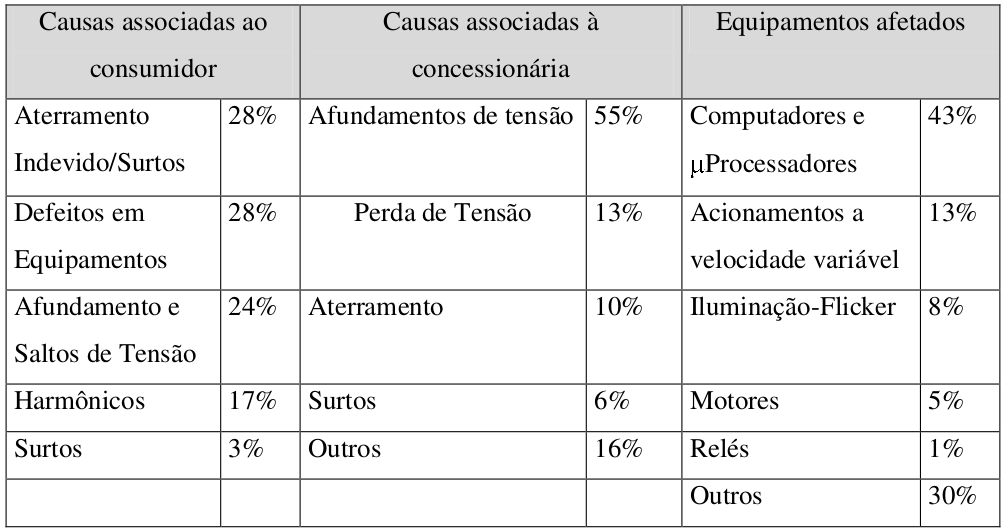
\includegraphics[width=12cm]{imagens/tab2-cap2.png}
\par{\small Fonte: Ribeiro, P., Workshop on Power Quality, II SBQEE, nov. 1997, citado por \cite{ALV10}.}
\label{fig:tabpertcons}
\end{center}
\end{table}
\par
Também segundo \cite{ALV10}, afundamento de tensão é a perturbação número um entre as perturbações que afetam a QEE na indústria. Menos severo e mais comum do que uma interrupção momentânea (corte total da tensão na carga), o afundamento pode causar o mesmo dano. Ambos podem causar interrupções de alguns equipamentos e até mesmo do processo inteiro.
% tabela 3
\begin{table}[!h]
\begin{center}
\caption{Perdas Financeiras em Grandes Consumidores Industriais e Comerciais (Interrupções e Afundamentos de Tensão)}
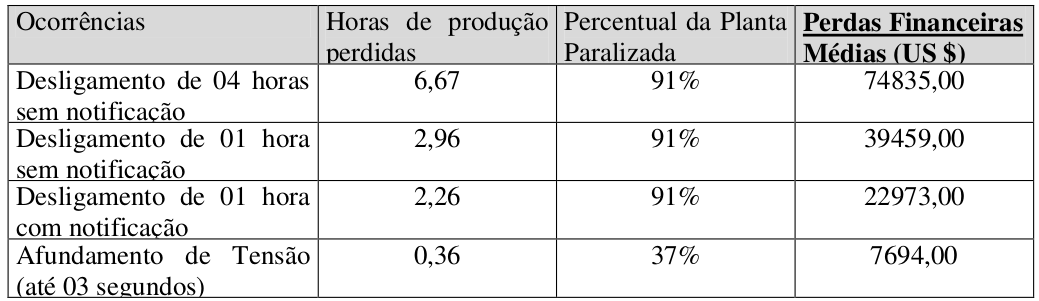
\includegraphics[width=12cm]{imagens/tab3_cap2.png}
\par{\small Fon11te:Valores médios, USA. Pesquisa realizada no início dos anos 90, citado por \cite{ALV10}.}
\label{fig:tabperdas}
\end{center}
\end{table}
\par
É economicamente inviável eliminar todas as faltas do sistema elétrico, para não haver afundamentos de tensão, e em contra partida não é eficaz reduzir o número de afundamentos se o custo por essa ação for maior do que o prejuízo causado pelos mesmos.
Às vezes, existem soluções simples a serem aplicadas como mudanças nas especificações dos equipamentos para gerar uma redução significativa no número de interrupções de equipamentos e/ou processos.
\par
Devido à generalidade dos parâmetros envolvidos (características do sistema elétrico, das cargas, do tipo de falta e proteção), o afundamento de tensão é um problema de análise complexa. Onde esta requer um conhecimento das características do distúrbio, informações estatísticas, probabilidade de ocorrência do afundamento, sensibilidade dos equipamentos e, informações do prejuízo causado pelo distúrbio \cite{ALV10}.
\par
Quanto à sensibilidade dos Equipamentos aos Afundamentos, \cite{ALV10} explicita que as cargas mais vulneráveis aos afundamentos são os equipamentos eletrônicos à base de microprocessadores, como os AVV e os CLP. 
\par
Disfunções nos CLPs ou nos microprocessadores (µP) de controle causam interrupções de parte ou de todo o processo, atuação da proteção dos AVVs e o seu desligamento, desatracamento das bobinas de contadores e relés auxiliares, perda de programação dos (µP) etc. Isto causa perda de produtividade, redução da qualidade do produto e diminuição da satisfação do cliente.
\par 
As explanações sobre a regulamentação, normativas e diretamente os índices da QEE introduzem e motivam o entendimento das causas motivadoras (distúrbios eletromagnéticos) para estudar e trabalhar com a QEE. Além disso, os conceitos abordados nesse capítulo possuem um papel não somente de referencial teórico para o trabalho proposto, mas também possibilitam uma base de entendimento para as futuras analises de dados no qual o sistema proposto trabalhara outomassivamente.